\documentclass[class=article, crop=false]{standalone}

\begin{document}
\section{Partie 5 - Observateur - Contrôleur}
% TODO create one simulink file for each part to enable freely modification
% TODO create a config function for each part in other to improve code testing
% TODO all variables on the same place
% TODO return all in the function to save in workspace
On va maintenant utiliser l'état estimé par l'observateur dans le retour d'état. La loi de commande est donc de la forme:
\begin{equation}
    u(t) = u_{\text{ref}} - K \underbrace{(\hat{X}(t) - X_{\text{ref}})}_{\delta \hat{X}(t)}
\end{equation}
On pourra choisir le gain $K$ calculé en plaçant les valeurs propres en boucle fermée ou en minimisant le critère $J_{LQ}$.

\newpage
\subsection{Question 23}
\begin{exercise}
    Implémenter l'observateur-contrôleur dans le modèle Simulink. Vérifier qu'il permet bien d'estimer l'état et de stabiliser la Balle sur la position $r_{\text{ref}} = 0$ avec un état initial suffisamment proche de l'équilibre pour que le linéarisé tangent reste une approximation valable.
\end{exercise}
\begin{resolution}
    \begin{figure}[H]
        \centering
        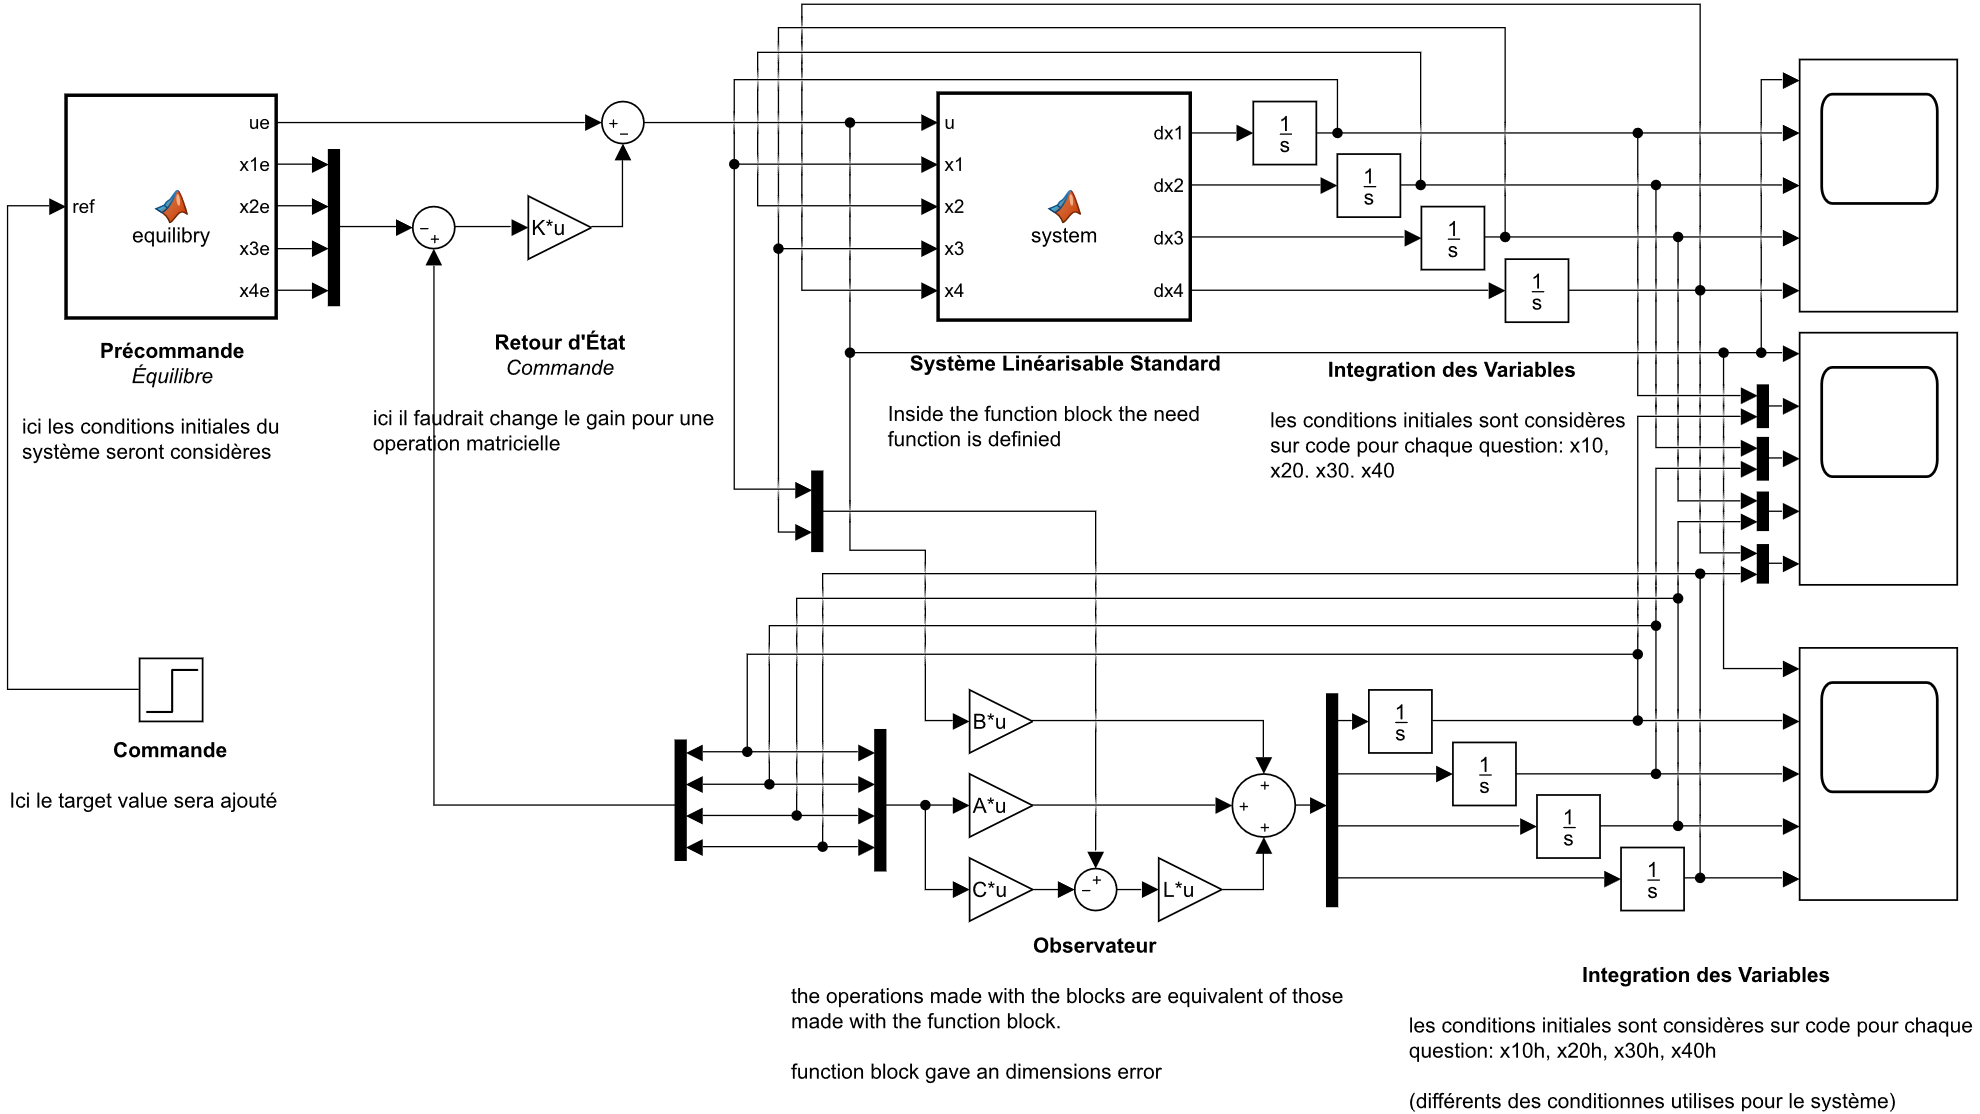
\includegraphics[width=0.8\textwidth]{../images/system_simulink_5.png}
        \caption{}
    \end{figure}
    \begin{figure}[H]
        \centering
        \begin{subfigure}[b]{0.475\textwidth}
            \centering
            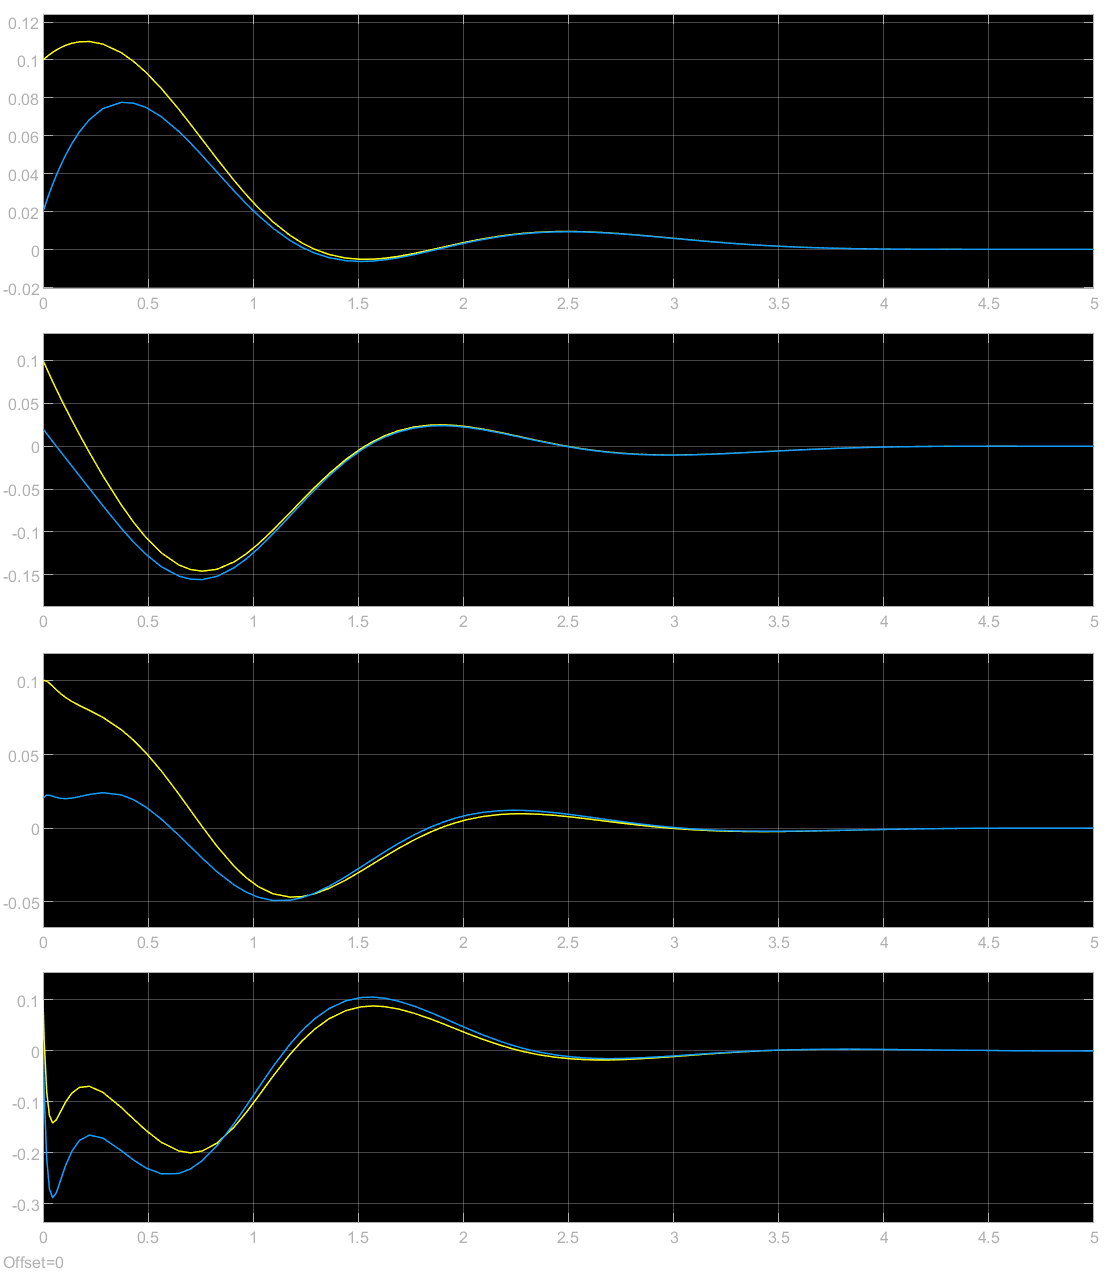
\includegraphics[width=\textwidth]{../images/simulink_scope5_0_1_02.png}
            \caption{}
        \end{subfigure}
        \begin{subfigure}[b]{0.475\textwidth}
            \centering
            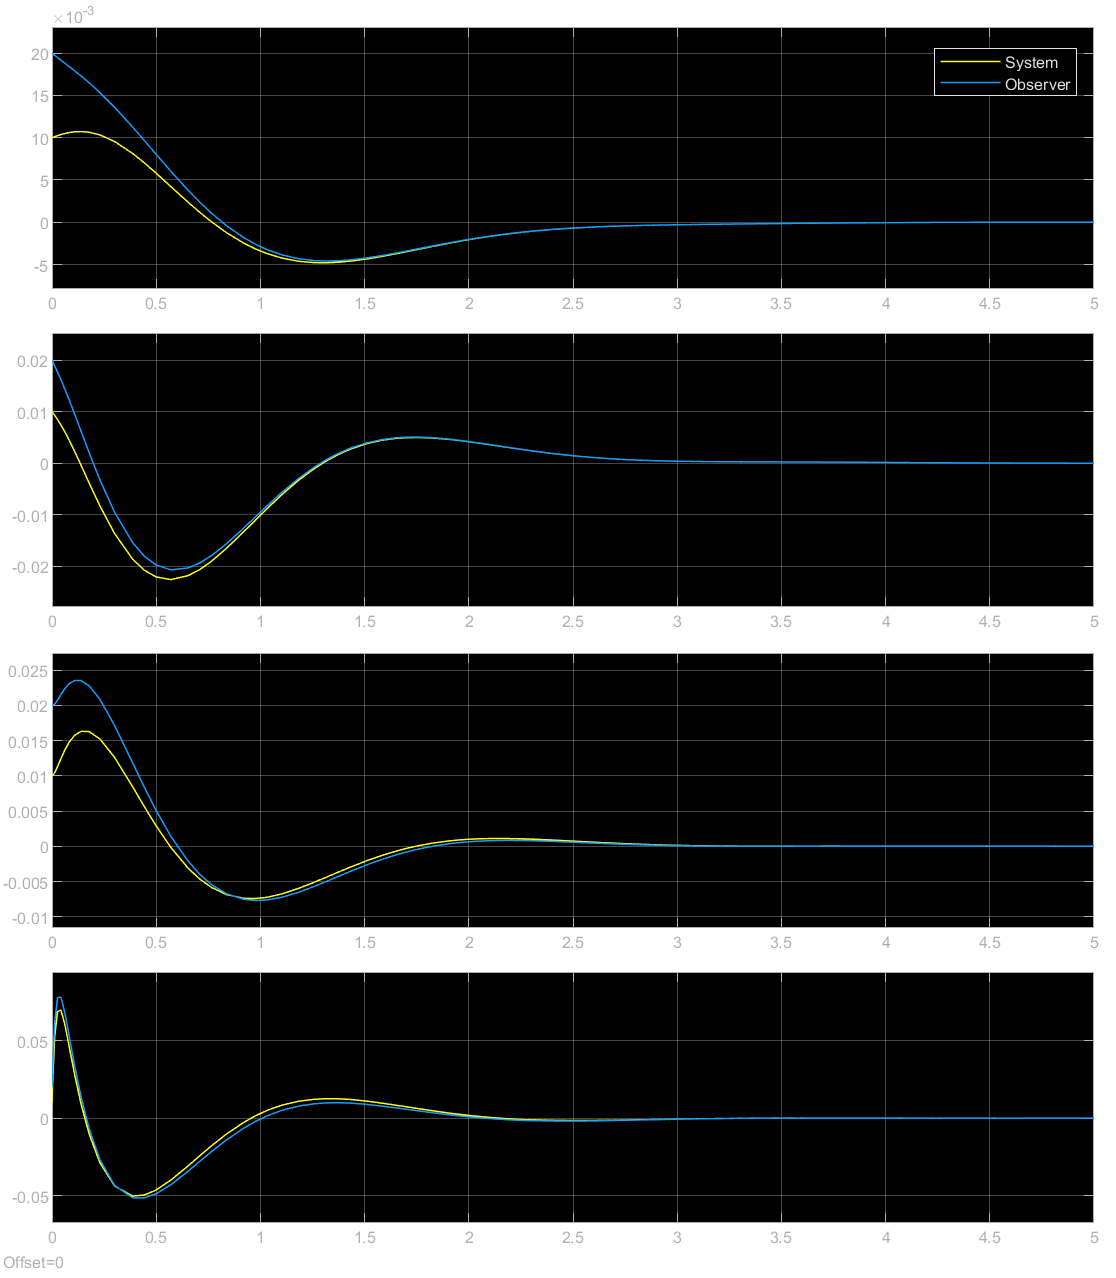
\includegraphics[width=\textwidth]{../images/simulink_scope5_0_01_02.png}
            \caption{}
        \end{subfigure}
        \caption{}
    \end{figure}
\end{resolution}

\newpage
\subsection{Question 24}
On souhaite maintenant stabiliser la Balle sur une position $r_{\text{ref}} \neq 0$ mais supposée suffisamment proche de 0 pour que le linéarisé tangent reste une approximation valable.
\begin{exercise}
    Compléter l'observateur-contrôleur dans le modèle Simulink afin de pouvoir estimer l'état et stabiliser la Balle sur n'importe quelle position $r_{\text{ref}} \neq 0$ supposée proche de 0. Vérifier qu'il permet bien d'estimer l'état et de stabiliser la Balle sur la position $r_{\text{ref}} \neq 0$ avec un état initial suffisamment proche de l'équilibre pour que le linéarisé tangent reste une approximation valable.
\end{exercise}
\begin{resolution}
    \begin{figure}[H]
        \centering
        \begin{subfigure}[b]{0.475\textwidth}
            \centering
            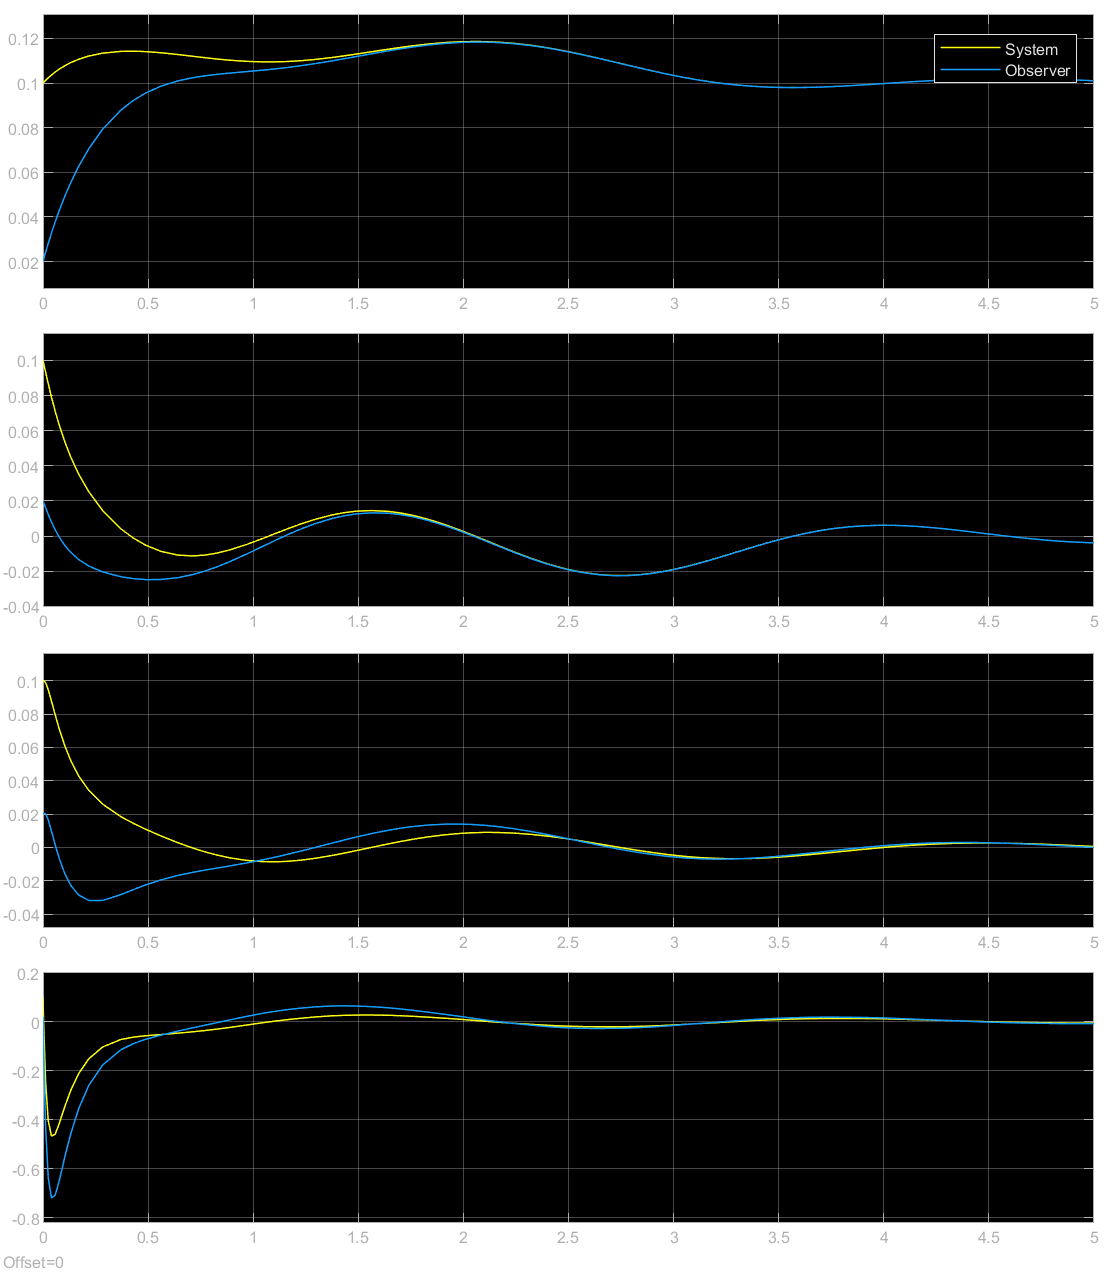
\includegraphics[width=\textwidth]{../images/simulink_scope5_01_1_02.png}
            \caption{}
        \end{subfigure}
        \begin{subfigure}[b]{0.475\textwidth}
            \centering
            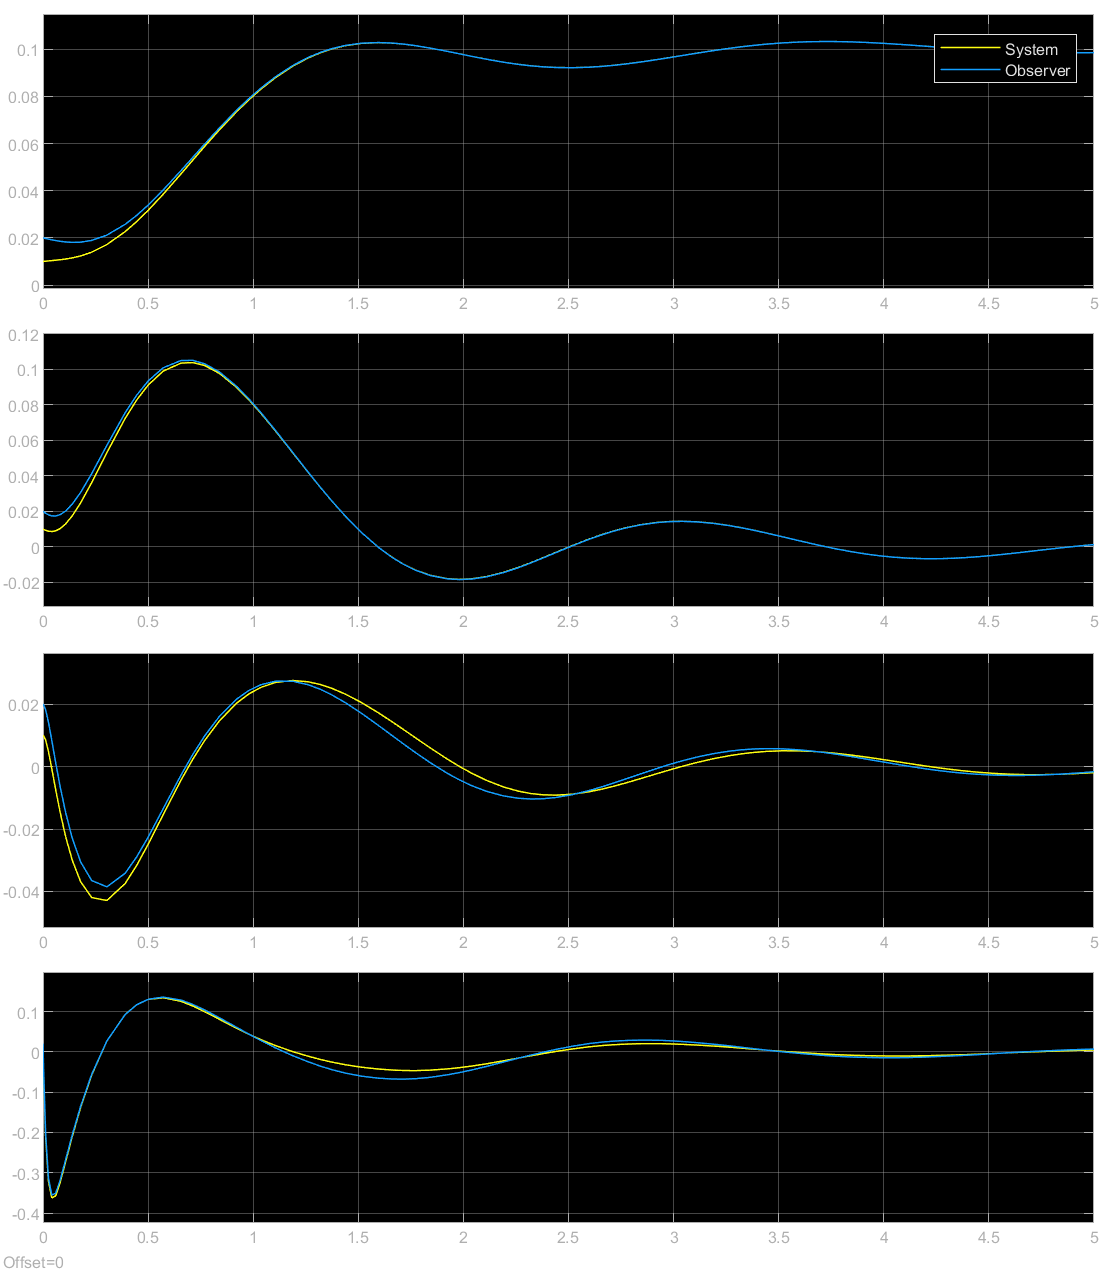
\includegraphics[width=\textwidth]{../images/simulink_scope5_01_01_02.png}
            \caption{}
        \end{subfigure}
        \caption{}
    \end{figure}
\end{resolution}

\newpage
\subsection{Question 25}
\begin{exercise}
    L'observateur-contrôleur est-il toujours performant lorsque la Balle s'éloigne significativement de la position $r_{\text{ref}} = 0$?
\end{exercise}
\begin{resolution}
    \begin{figure}[H]
        \centering
        \begin{subfigure}[b]{0.475\textwidth}
            \centering
            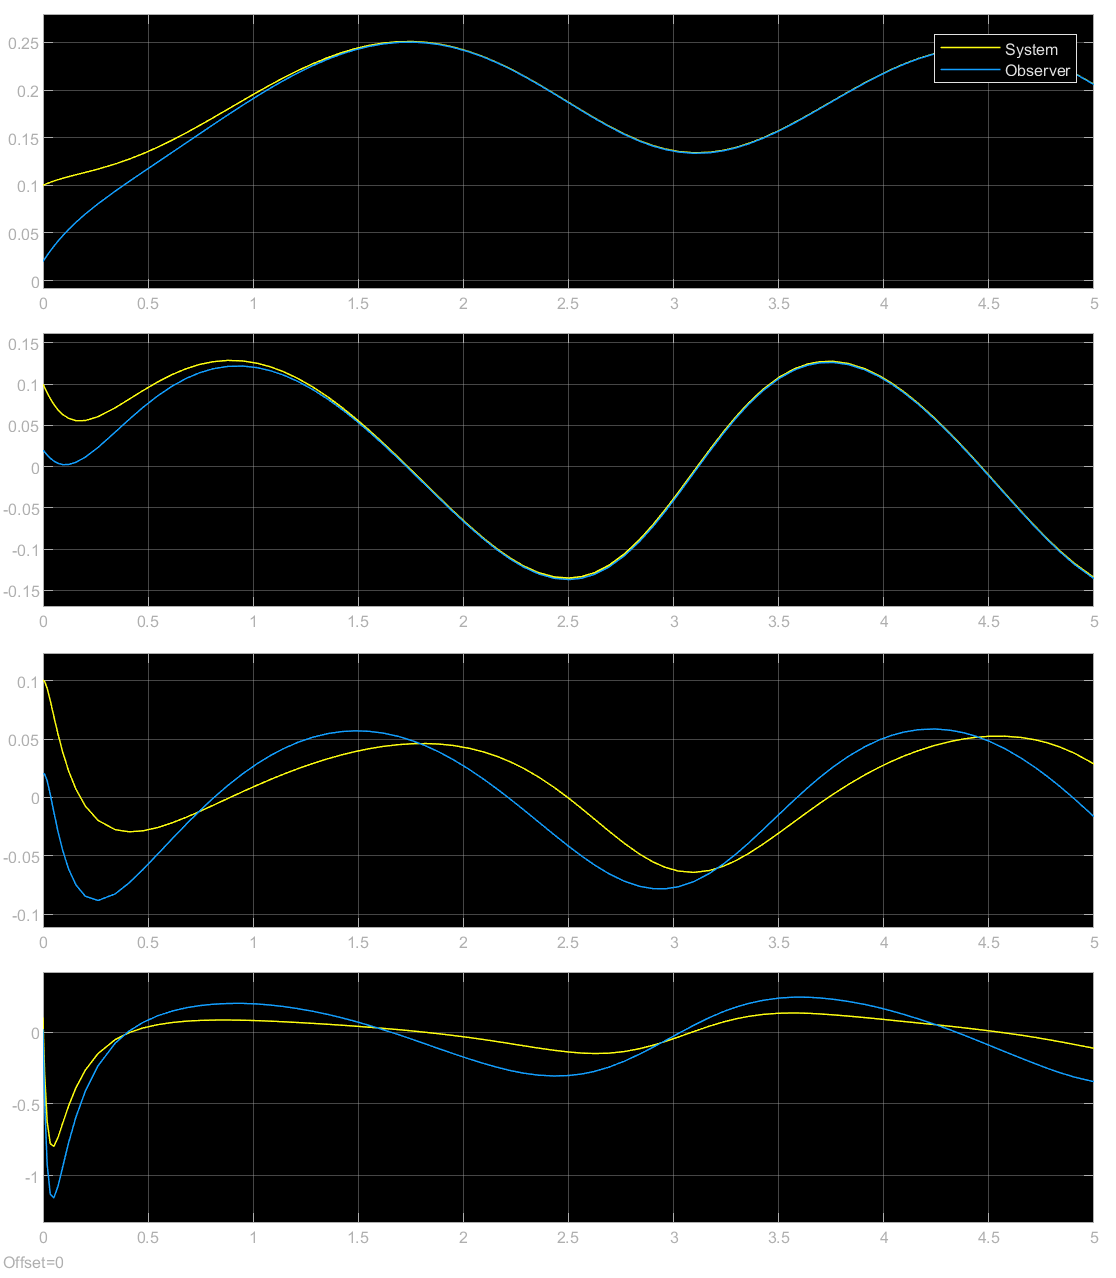
\includegraphics[width=\textwidth]{../images/simulink_scope5_02_1_02.png}
            \caption{}
        \end{subfigure}
        \begin{subfigure}[b]{0.475\textwidth}
            \centering
            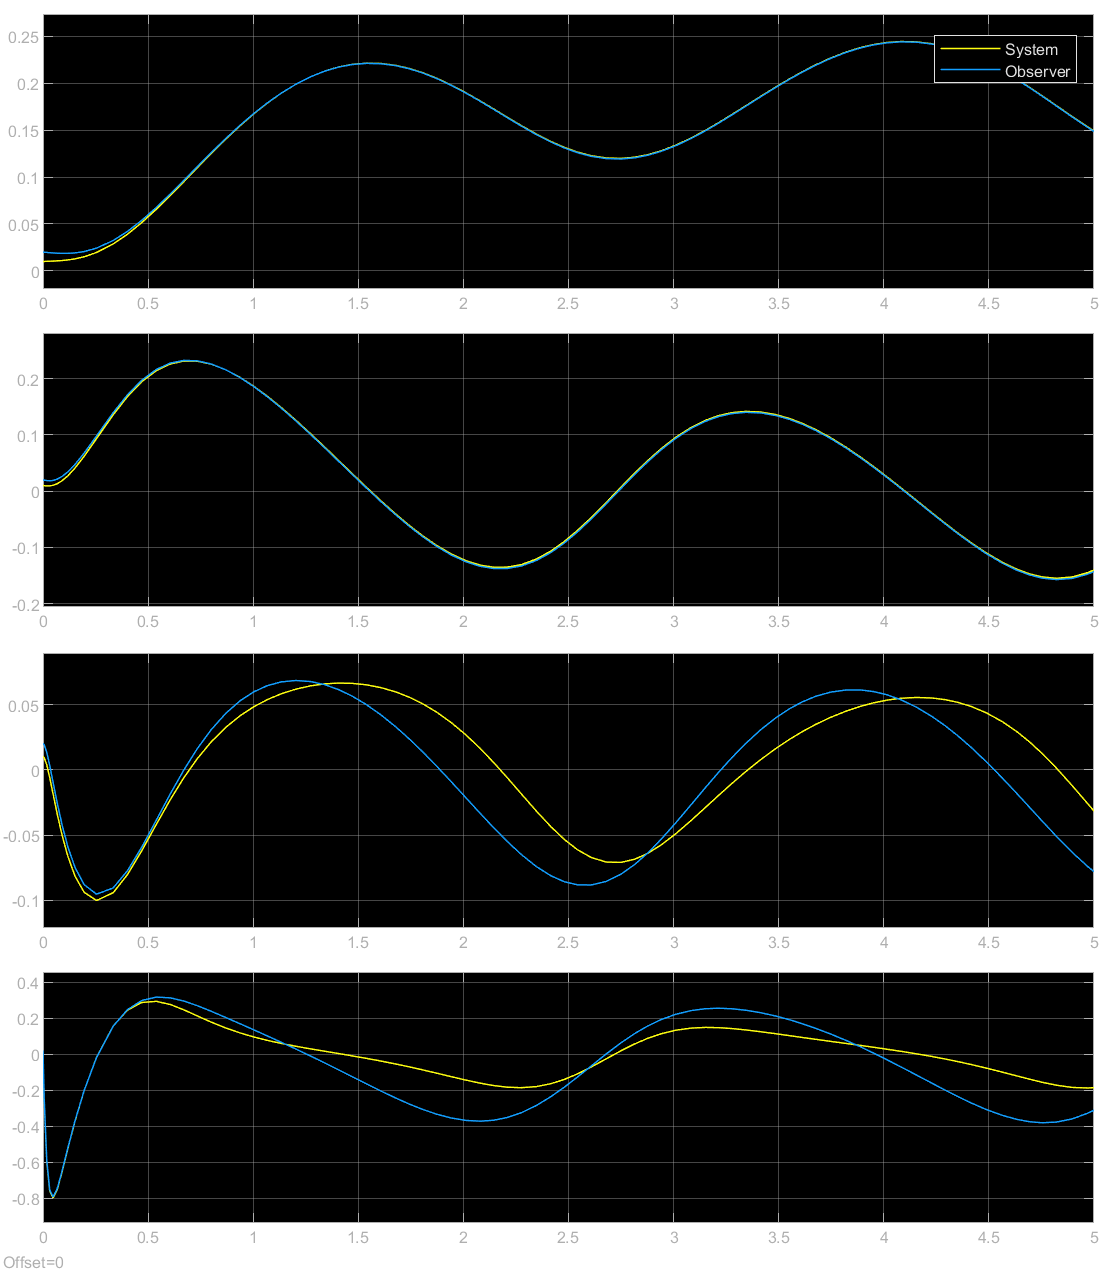
\includegraphics[width=\textwidth]{../images/simulink_scope5_02_01_02.png}
            \caption{}
        \end{subfigure}
        \caption{}
    \end{figure}
\end{resolution}
\end{document}